\documentclass[crop,tikz,convert={outext=.svg,command=\unexpanded{pdf2svg \infile\space\outfile}},multi=false]{standalone}[2012/04/13]

\usepackage[utf8]{inputenc}
\usepackage{amsmath, amssymb}
\usepackage{pgfplots}

%-------------------------------------
% Tikz and pgf options & definitions
%-------------------------------------
\pgfplotsset{compat=1.15}
\pgfmathsetseed{1}

\usetikzlibrary{positioning}
\usetikzlibrary{shapes}
\usetikzlibrary{backgrounds, fit}
\usetikzlibrary{calc}
\usetikzlibrary{decorations.markings}
\usetikzlibrary{matrix}

\def\colorvector at (#1,#2,#3){
\coordinate (A) at (#1, #2);
\filldraw[draw=black,fill=test!!+] (A)++(0,0) rectangle ++(0.25,0.25) node (A0) {};
\filldraw[draw=black,fill=test!!+] (A)++(0.3,0) rectangle ++(0.25,0.25) node (A1) {};
\filldraw[draw=black,fill=test!!+] (A)++(0.6,0) rectangle ++(0.25,0.25) node (A2) {};
\node[right=of A2, xshift=-7.5ex, yshift=-0.75ex] {$\ldots$};
\filldraw[draw=black,fill=test!!+] (A)++(1.5,0) rectangle ++(0.25,0.25) node (A4) {};
\node[left=of A1, xshift=4.4ex, yshift=-0.75ex] (BEG\i) {$#3=[$};
\node[right=of A4, xshift=-8ex, yshift=-0.75ex] (END\i) {$]^{T}$};
}

\begin{document}
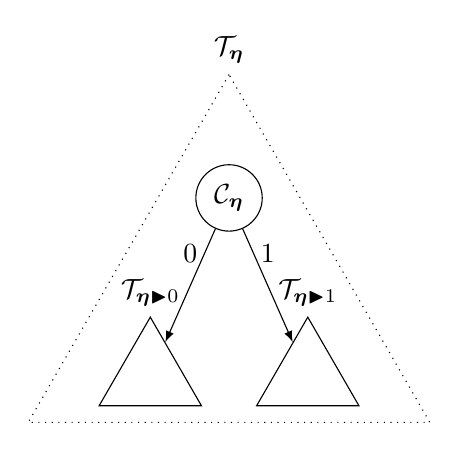
\begin{tikzpicture}[
edge from parent/.style={draw,-latex},
level distance=15mm,
level 1/.style={sibling distance=20mm},
level 2/.style={sibling distance=30mm},
level 3/.style={sibling distance=15mm},
level 4/.style={sibling distance=15mm}
]

\usetikzlibrary{shapes}
\tikzstyle{c} = [draw, shape=circle]
\tikzstyle{r} = [draw, shape=rectangle,minimum width=10mm]
\tikzstyle{tr} = [draw, regular polygon, regular polygon sides=3, anchor=north, minimum width=1.5cm]

\node[c] (r) {${\cal C}_{\boldsymbol{\eta}}$}[edge from parent]
    child {node[tr, label=above:{${\cal T}_{\boldsymbol{\eta} \blacktriangleright 0}$}] (t0) {}
        edge from parent coordinate (e0);
    }
    child {node[tr, label=above:{${\cal T}_{\boldsymbol{\eta} \blacktriangleright 1}$}] (t1) {}
        edge from parent coordinate (e1);
    };
% code labels
\node at([yshift=4mm]e0) {0};
\node at([yshift=4mm]e1) {1};

\node[fit={(e0)(e1)(t0)(t1)}, draw, yshift=5mm, dotted, inner sep=-4mm, regular polygon, regular polygon sides=3,label=above:{${\cal T}_{\boldsymbol{\eta}}$}](X){};
\end{tikzpicture}
\end{document}